\section{Waves and sound}
\label{s:waves}

\bi
\i Sound is an example of a pressure wave that propagates 
from one location to another---e.g., from an instrument to 
our ears.

\i In this section, we learn about general properties of 
waves, with applications to sound.

\ei

%%%%%%%%%%%%%%%%%%%%%%%%%%%%%%%%%%%%%%%%%%%%%%%%%%%%%
\subsection{Basic definitions}

\bi
\i Wave: any `disturbance' that transports energy
and momentum from one location to another without
the transport of matter.

\i \ex surface water waves, waves on a stretched string, 
pressure waves in a column of air in a tube,
electromagnetic waves (light, radio waves, X-rays, ...), 
sound waves in air, 
the `wave' at a football game, ...

\i Waves can propagate 
in one dimension (e.g., along a stretched string or in a column of air), 
in two dimensions (e.g., along the surface of a pond or
the head of a drum), or 
in three dimensions (e.g., through air or even empty space).

\i Wave motion is different from particle motion.
The disturbance propagates, not the individual particles.

\i The {\em intensity} of a wave is the rate at which energy
passes through a unit area perpendicular to the direction
of propagation.
(Units: ${\rm W}/{\rm m}^2$ corresponding to 
${\rm energy}/({\rm area}\cdot{\rm time})$.)
For a spherical wave in three dimensions, the intensity is
proportional to $1/r^2$, where $r$ is the distance from the
source of the wave.

\i Although most waves require a medium in which to travel
(for example, sound), some waves do not.
Electromagnetic waves, like light, can travel through empty
space.

\i \ex A ringing bell in a vacuum jar.
(You can see the bell, but you can't hear the sound.)

\i Transverse wave: 
the disturbance is perpendicular to the direction of 
wave propagation.

\i Longitudinal (or compressional) wave: 
the distubance is parallel to the direction of 
wave propagation.

\i Electromagnetic waves, like light, are examples
of transverse waves.

\i Sound is an example of a longitudinal pressure wave 
consisting
of alternating compressions (overdensities) 
and expansions (underdensities) in a medium.
The medium can be air (or any gas), a liquid, or a solid.

\i Liquids and gases can only support 
longitudinal waves, since there is no ``sideways" 
restoring force.
(The reason why surface water waves can have a 
transverse component is gravity is acting as the
restoring force.)

\i \demo Illustrate transverse and longitudinal waves on a slinky.
Illustrate the difference between a wave pulse and 
a periodic wave on a slinky.

\ei

%%%%%%%%%%%%%%%%%%%%%%%%%%%%%%%%%%%%%%%%%%%%%
\subsection{Wave velocity}

\bi

\i Since the wave disturbance propagates from one location 
to another, waves have a velocity equal to the distance
traveled by a the disturbance divided by the corresponding time
interval.

\i The wave velocity depends only on the properties of
the medium and not on the motion of the source relative
to the medium.

\i Wave velocity on a string: 
%
\be
v=\sqrt{F/\mu}
\ee
%
where $F$ is the tension in the string and $\mu=m/L$ is the
mass per unit length of the string.

\i The tension in the string is the restoring force that
tries to bring the (slightly) deformed string back to its equilibrium
position.
Note that for a heavier string, the wave velocity is
less than that for a light string, assuming the same tension.

\i More generally, the wave velocity in any medium is
given by 
%
\be
v=\sqrt{{\rm elastic}/{\rm inertial}}
\ee
%
where the elastic property of the medium provides the restoring 
force and the inertial property provides the resistance that 
the medium offers to changes in its state of motion.

\i Using this more general expression, one can show that 
the speed of sound in air depends on the temperature of 
the air:
%
\be
v_{\rm air} = 331~{\rm m/s}\,
\sqrt{1 + \frac{T_C}{273.15}}
\ee
%
where $T_C$ is the temperature in degrees Celsius 
(centigrade scale).

\i \exer Show that speed of sound in air at room temperature
$T=25~{}^\circ{\rm C}$ ($77~{}^\circ{\rm F}$) is given by
%
\be
v_{\rm air} = 346~{\rm m/s}
\ee

\i \exer Compare the above answer to the speed of sound in
air at $T=20~{}^\circ{\rm C}$ ($68~{}^\circ{\rm F}$).
Show that the percent difference between the two speeds is
approximately $1\%$, which (as we will show in the next subsection)
corresponds to a $1\%$ increase in the frequency (or pitch)
of a sound.

\i Sound travels in other materials as well.
For example, 
%
\begin{align}
v_{\rm water} \approx 1440~{\rm m/s}\,,
\quad
v_{\rm steel} \approx 5000~{\rm m/s}
\end{align}

\ei

%%%%%%%%%%%%%%%%%%%%%%%%%%%%%%%%%%%%%%%%%%%%%%%%%%%%%
\subsection{Periodic waves}

\bi

\i Periodic waves are produced by periodic sources.
They are characterized by frequency $f=1/T$, amplitude $A$, and
wavelength $\lambda$ (the distance between two like points on the
wave).
The waves travel with wave speed $v$ given by 
%
\be
v=\frac{\lambda}{T} = f\lambda
\ee

\i Sound waves can be produced in principle at any frequency,
but the human ear is sensitive ``only" to frequencies
in the approximate range 20~Hz to 20,000~Hz.
Dogs can hear higher frequencies;
whales and elephants, lower frequencies.

\i \exer Show that the corresponding wavelengths of
sound waves in air traveling with $v=346~{\rm m/s}$ 
for $f=20~{\rm Hz}$ and 20,000~Hz are 
$\lambda = 17~{\rm m}$ and 1.7~cm, respectively.
(We will refer to these numbers later on when we talk 
about the diffraction of sound waves around obstacles.)

\i The intensity for a periodic wave is proportional to 
the wave velocity,
the square of the displacement wave amplitude, 
and the square of its frequency.

\i The human ear is sensitive to intensities ranging
from $10^{-12}~{\rm W/m}^2$ (threshold of hearing) to
$1~{\rm W/m}^2$ (threshold of pain).

\i The maximum displacement of the air molecules corresponding
to these two intensities at a frequency of 1000~Hz are
$1.1\times 10^{-11}~{\rm m}$ and $1.1\times 10^{-5}~{\rm m}$,
respectively.
Note that the maximum displacement of the air molecules at
the threshold of hearing is approximately $1/10$ the
size of a typical atom!!

\i The maximum pressure deviations due to the over- and 
underdensity of the air molecules are
$2.8\times 10^{-5}~{\rm Pa}$ and $28~{\rm Pa}$, respectively.
These numbers should be compared to the ambient atmospheric
pressure of $1\times 10^5~{\rm Pa}$.
Thus, even the maximum pressure deviations at the threshold 
of pain are approximately
10,000 times smaller than the ambient atmospheric pressure.

\i The above items illustrate the incredible sensitivity 
of the human ear to hear sound.

\i Simple harmonic waves are produced by SHM sources.
In 1-dimension, a plot of a simple harmonic wave has
sinusoidal dependence with respect to both:
(i) variable position $x$ for fixed $t$ (e.g., a snapshot of the wave), 
and
(ii) variable time $t$ for fixed $x$ (simple harmonic displacement of 
the particle at $x$).

\i Mathematically, a simple harmonic wave in 1-dimension
has the form
%
\be
s(x,t) = s_m \,\sin
\left[2\pi\left(\frac{x}{\lambda}-\frac{t}{T}\right) - \phi_0\right]
\ee
%
Note the periodicity in the waveform when $x$ is 
increased by one wavelength 
$\lambda$ and $t$ is increased by one period $T$.

\i Note that when we plot air molecule displacement 
(or pressure deviation from atmospheric pressure) 
as a function of position $x$, we are giving
a `transverse-wave representation' of a longitudinal
wave.

\i \demo Graphical illustration that air molecule displacement
and pressure deviations are 90$^\circ$ out of phase with 
one another---i.e., one is maximum (or minimum) 
when the other is zero.

\ei

%%%%%%%%%%%%%%%%%%%%%%%%%%%%%%%%%%%%%%%%%%%%%%%%%%%%%%%%%
\subsection{Superposition principle and interference}

\bi

\i Principle of superposition:
The sum of two waves is another wave.

\i Waves can pass through one another and emerge without
changing the identity of the other wave.

\i Waves are said to {\em constructively} or {\em destructively} 
interfere when the disturbances in the two waves add or subtract 
from one another.

\i For two waves having the same frequency, whether the two
waves add constructively or destructively depends on the
{\em phase difference} between the two waves.

\i \demo Illustrate superposition of two sine waves using sumsines.m,
keeping the frequency the same, but varying the amplitude and 
phase of the two waves.

\i \ex Noise cancelling headphones use destructive interference 
to reduce the level of ambient noise.
(The headphones sense the ambient noise, invert the corresponding
sound waves, and then send the inverted wave to the earphones where 
they cancel most of the ambient noise.)

\i \demo Illustrate interference of waves traveling in two-dimensions
by overlaying two transparencies of concentric circles.
The clear spaces between the concentric circles represent the crests 
of the waves; the distance between two neighboring 
circles is one wavelength.
Constructive interference corresponds to clear areas of the overlaid 
transparencies.

Note that the number of radial lines corresponding to 
constructive interference decreases as the spacing between the two 
point sources decreases.

\i Beats are an example of two sound waves with nearly
the same frequencies $f_1$ and $f_2$ interfering with
one another.
The beat frequency is given by $f_{\rm beat} = |f_1-f_2|$.

\i Beats are an example of interference in time, as opposed to 
interference in space.

\i \demo Illustrate beats using two tuning forks having
frequencies of 440~Hz and 441~Hz.

We hear a sound with frequency 
$\bar f =(f_1+f_2)/2= 440.5~{\rm Hz}$, whose amplitude is 
modulated in time with frequency $f_{\rm beat}=|f_1-f_2|=1~{\rm Hz}$.

\i \demo Illustrate beats using sumsines.m
with same amplitudes, but $f_1=9~{\rm Hz}$ and $f_2=10~{\rm Hz}$.
Change the amplitude of one of the waves, noting how the 
modulation envelope changes---e.g., the modulation doesn't dip to
zero anymore.
Show how changing the phase of the two waves shifts the modulation
envelope to the right or to the left.

\i \demo Illustrate beats using the Faber Electroacoustics Toolbox
using two signal generator and the oscilloscope mode.
Set $f_1$ to $440~{\rm Hz}$ and let $f_2$ be variable.
Initially set $f_2=441~{\rm Hz}$ to hear beats with a frequency
of 1~Hz.
Adjust $f_2$ so that the beat frequency is too large to hear beats.
When do we eventually hear two {\em separate} frequencies?
What do we see using iSpectrum in spectrum analyzer mode for this case?

\i NOTE: 
We normally hear beats if the frequency difference is less 
than about 10~Hz, independent of the center frequency.
We can distinguish two separate frequencies (played simultaneously)
when the frequency
difference is greater than about 10\% of the center frequency,
which corresponds to about two semitones.

\ei

%%%%%%%%%%%%%%%%%%%%%%%%%%%%%%%%%%
\subsection{Standing waves}

\bi

\i Begin by considering waves on a string.

\i A right-moving wave becomes a left-moving wave
when it is reflected off of a boundary.
For a fixed end, the reflected wave is inverted;
for a free end, the reflected wave is not inverted.
(Note that the string at a fixed end has zero displacement,
so the incident and reflected waves on the string 
must be opposite one another in order to sum to 
zero at this point.)

This process also occurs at the left boundary, changing
a left-moving wave into a right-moving wave, etc.

\i The superposition of right and left-moving waves having
just the right frequencies 
can give rise to standing 
wave patterns on a string fixed at both ends:
%
\be
\lambda_n=\frac{2L}{n}\,,
\quad
f_n = \frac{v}{\lambda_n} = n\left(\frac{v}{2L}\right)\,,
\quad
n=1,2,\cdots
\ee
%
$n=1$ is the fundamental frequency; different values of 
$n$ correspond to different {\em harmonics}.

\i Draw standing wave patterns for a string fixed at both ends.

\i Nodes are locations where the displacement is zero.
Anti-nodes are locations where the displacement is maximum.

\i Note that standing waves are a resonance phenomenon.
Only for certain wave frequencies do the right-moving and left-moving
waves (which are traveling back-and-forth on the string) add 
constructively to the new waves that are produced at the source.
For other frequencies, the new waves destructively interfere with
the waves already traveling along the string.

\i \demo Produce standing waves on a long stringlike spring
by oscillating one end back-and-forth at the appropriate 
frequencies.

\i \demo Illustrate standing waves using standingwaves.m
with arguments 1, 2, 3, 1.7.
Compare the amplitude of the summed waves on and off resonance.

\i Standing wave vibrations in a column of air
can also be set up in a cylindrical tube.

Tube open at both ends:
%
\be
\lambda_n = \frac{2L}{n}\,,
\quad
f_n = n\left(\frac{v}{2L}\right)\,,
\quad n=1,2,3, \cdots
\ee
%

Tube open at one end, closed at the other:
%
\be
\lambda_n = \frac{4L}{n}\,,
\quad
f_n = n\left(\frac{v}{4L}\right)\,,
\quad n=1,3,5, \cdots
\ee
$n=1$ is the fundamental frequency.

\i Draw standing wave patterns for both types of
tubes.
Compare plots of pressure deviation and air molecule
displacement as functions of distance along the tube.
(See Figure~\ref{f:displacement-pressure}.)
Recall that they are 90$^\circ$ out of phase with one another.
For example, an open end corresponds to a node for 
pressure deviation but an anti-node for air molecule displacement.
%
\begin{figure}[htbp]
  \begin{center}
  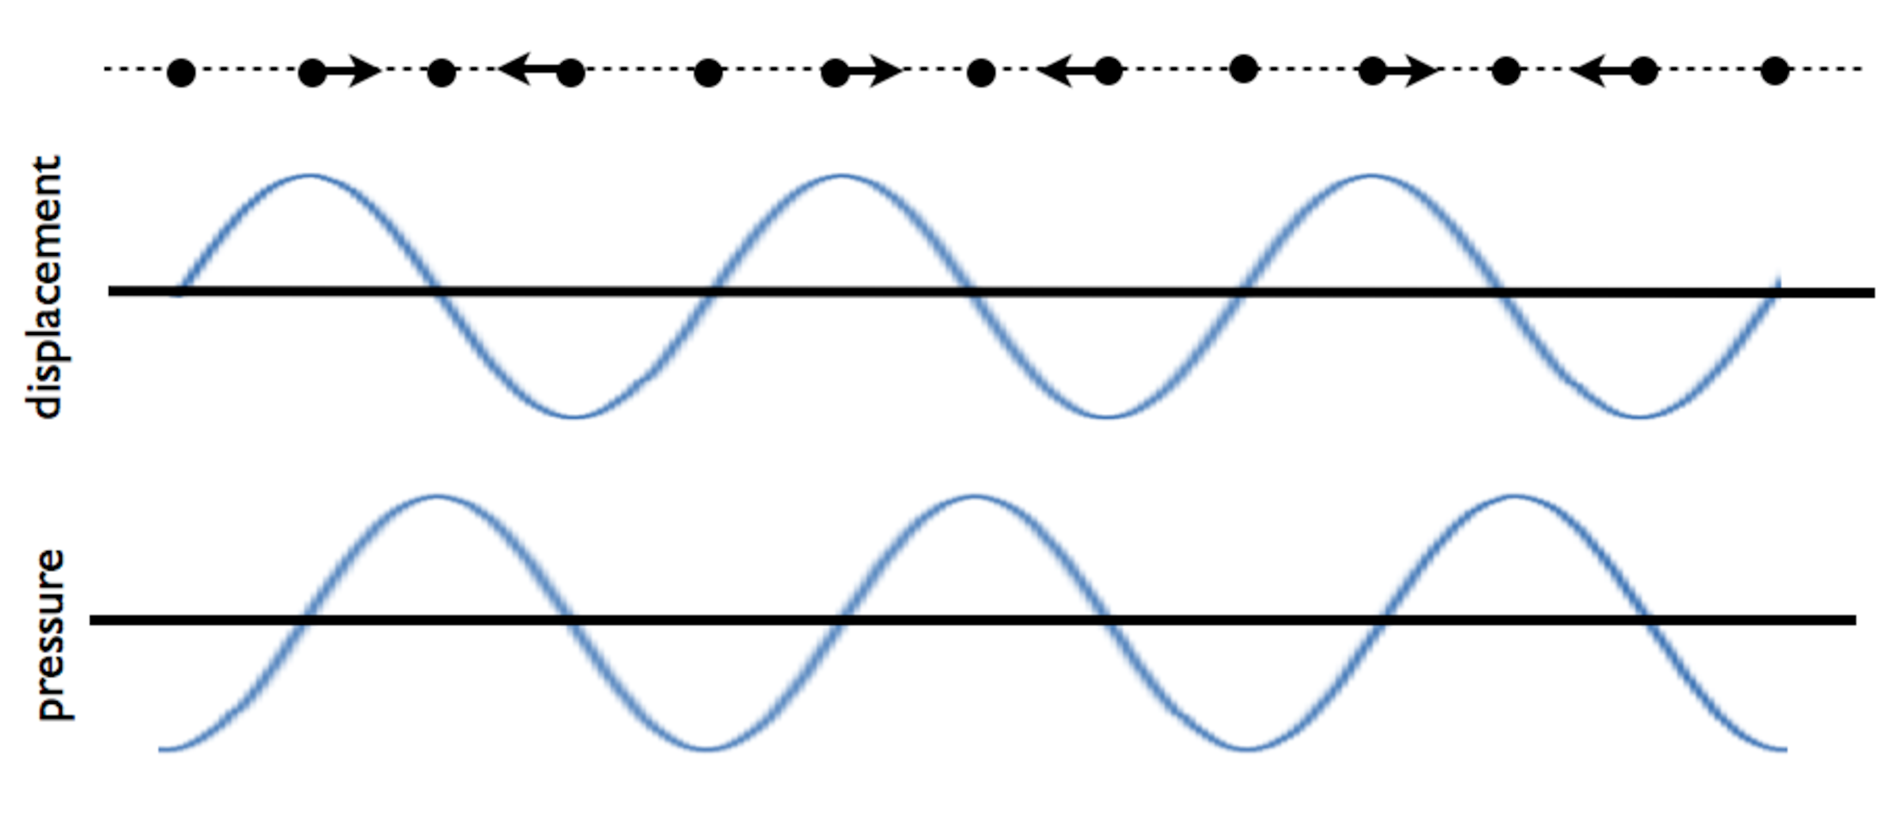
\includegraphics[width=.9\textwidth]{displacement-pressure.pdf}
  \caption{Relationship between air molecule displacement and pressure deviation.}
  \label{f:displacement-pressure}
  \end{center}
\end{figure}

\i Note that a tube open at both ends has both odd
and even harmonics, while a tube closed at one 
end has only odd harmonics.

\i Although it is also possible to consider standing 
waves in a tube closed at both ends (which has the 
same standing wave patterns as a
tube open at both ends), it is of no interest for us
in the context of sound, since the waves in the tube
have no way to couple their oscillations to the air
outside the tube.
 
\i \ex A clarinet is woodwind instrument that 
behaves like a tube closed at one end.
(The reed corresponds to the closed end.)
The notes it produces are dominated by odd harmonics.

\i \ex Contrast the clarinet to a 
flute or recorder, which behave like tubes open
at both ends.
These instruments produce notes that have both
odd and even harmonics.

\i The standing wave patterns for a cylindrical 
tube with one or two open ends actually have their 
pressure nodes at a slight distance {\em outside} 
the tube, due to the two-dimensional nature of the cylinder.
If $R$ denotes the radius of the cylinder:
%
\begin{align}
&L_{\rm eff} = L + 0.61 R
\quad
({\rm tube\ open\ at\ one\ end})
\\
&L_{\rm eff} = L + 1.22 R
\quad
({\rm tube\ open\ at\ both\ ends})
\end{align}
%
is the effective length of the tube.
To be accurate, the effective length should be 
used in the expressions for the standing wave
wavelengths and frequencies.

\i \demo Using a tuning fork with frequency
$f=1024~{\rm Hz}$ and an adjustable length tube 
that is closed at one end,
estimate the speed of sound in air.

Find two consecutive lengths of the tube that 
resonate with the tuning fork.
The difference of those two lengths,
$\Delta L = L_2-L_1$, 
must equal half a wavelength $\lambda$, so
$\lambda = 2\Delta L$.
But since $v=f\lambda$, we have
%
\be
v = 2f(L_2-L_1)
\ee
%
as our estimate of the speed of sound in air.
(Compare this to $v_{\rm air}=346~{\rm m/s}$ at room temperature.)

\i One can also talk about standing waves for two-dimensional
objects (e.g., a stretched drum head) and for stiff objects
like one-dimensional bars and two-dimensional plates.

\i For these more complicated objects, the frequencies
corresponding to different standing wave patterns do 
{\em not} form a simple harmonic series.

\i \demo 
Connect a loudspeaker to a function generator, whose frequency 
can be varied.
Attach a Chladni plate to the speaker, and sprinkle salt on 
the plate.
Adjust the frequency of the function generator
to find the resonant frequencies for
different standing wave patterns of the plate.
(The salt collects along the nodal lines of the standing wave
patterns.)
Record the resonant frequencies and show that they are not 
harmonically related to one another.

\ei

%%%%%%%%%%%%%%%%%%%%%%%%%%%%%%%%%%%%%%%%%%%%%%%%%%%%%%%%%
\subsection{Reflection}
\bi

\i When a wave travels from one medium to another, 
part of the wave is transmitted and part of the wave 
is reflected.

\i For a wave traveling in one-dimension (like a 
wave on a string, or a sound wave in a column of air),
the reflected wave moves in the direction opposite
to the incident wave.

\i The reflected wave is inverted 
(i.e., has a $180^\circ$ phase shift relative to
the incident wave) if the incident wave encounters 
a fixed end.
The reflected wave has the same shape
(i.e., there is no phase shift relative to the 
incident wave) if the incident
wave  encounters a free end.

\i \demo Illustrate this by observing
incident and reflected waves on a single
stretched string, with fixed or free ends.

\i For waves traveling in two- or three-dimensions,
the wavefronts are approximately lines or planes
far from the source.
The direction of wave propogation is perpendicular to
the wave fronts (it is called a {\em ray}.)

\i The {\em law of reflection} tells how the direction 
of the reflected wave is related to the direction of the 
incident wave:
%
\be
\theta_i = \theta_r
\ee
%
where $\theta_i$, $\theta_r$ are the angles that the 
incident and reflected waves make with respect to 
the normal.

\i Reflection is responsible for echoes.
Reducing the amount of echoes is important
in the design of musical performing halls.

\i \ex A whispering room in a science museum consists 
of two parabolic walls facing one another, which focus 
sound produced at one focal point to the other focal point.

\ei

%%%%%%%%%%%%%%%%%%%%%%%%%%%%%%%%%%%%%%%%%%%%%%%%%%%%%%%%%
\subsection{Refraction}
\bi

\i Refraction is the `bending' or change in the 
direction of propagation of a wave as it passes from
one medium into another.
The amount of bending depends on the wave velocities 
in the two media.

\i \demo A straw in a glass of water appears to be
`bent' when viewed from an angle.

\i The {\em law of refraction} (Snell's law) 
tells how the direction of the transmitted wave is 
related to the direction of the incident wave:
%
\be
\frac{\sin\theta_1}{v_1} = \frac{\sin\theta_2}{v_2}
\ee
%
where $v_1$, $v_2$ are the velocities of the waves in 
the two media.
(Fig.~\ref{f:refraction}).  
The angle with respect to the normal is larger in the 
medium with the larger wave velocity.
%
\begin{figure}[htbp]
  \begin{center}
  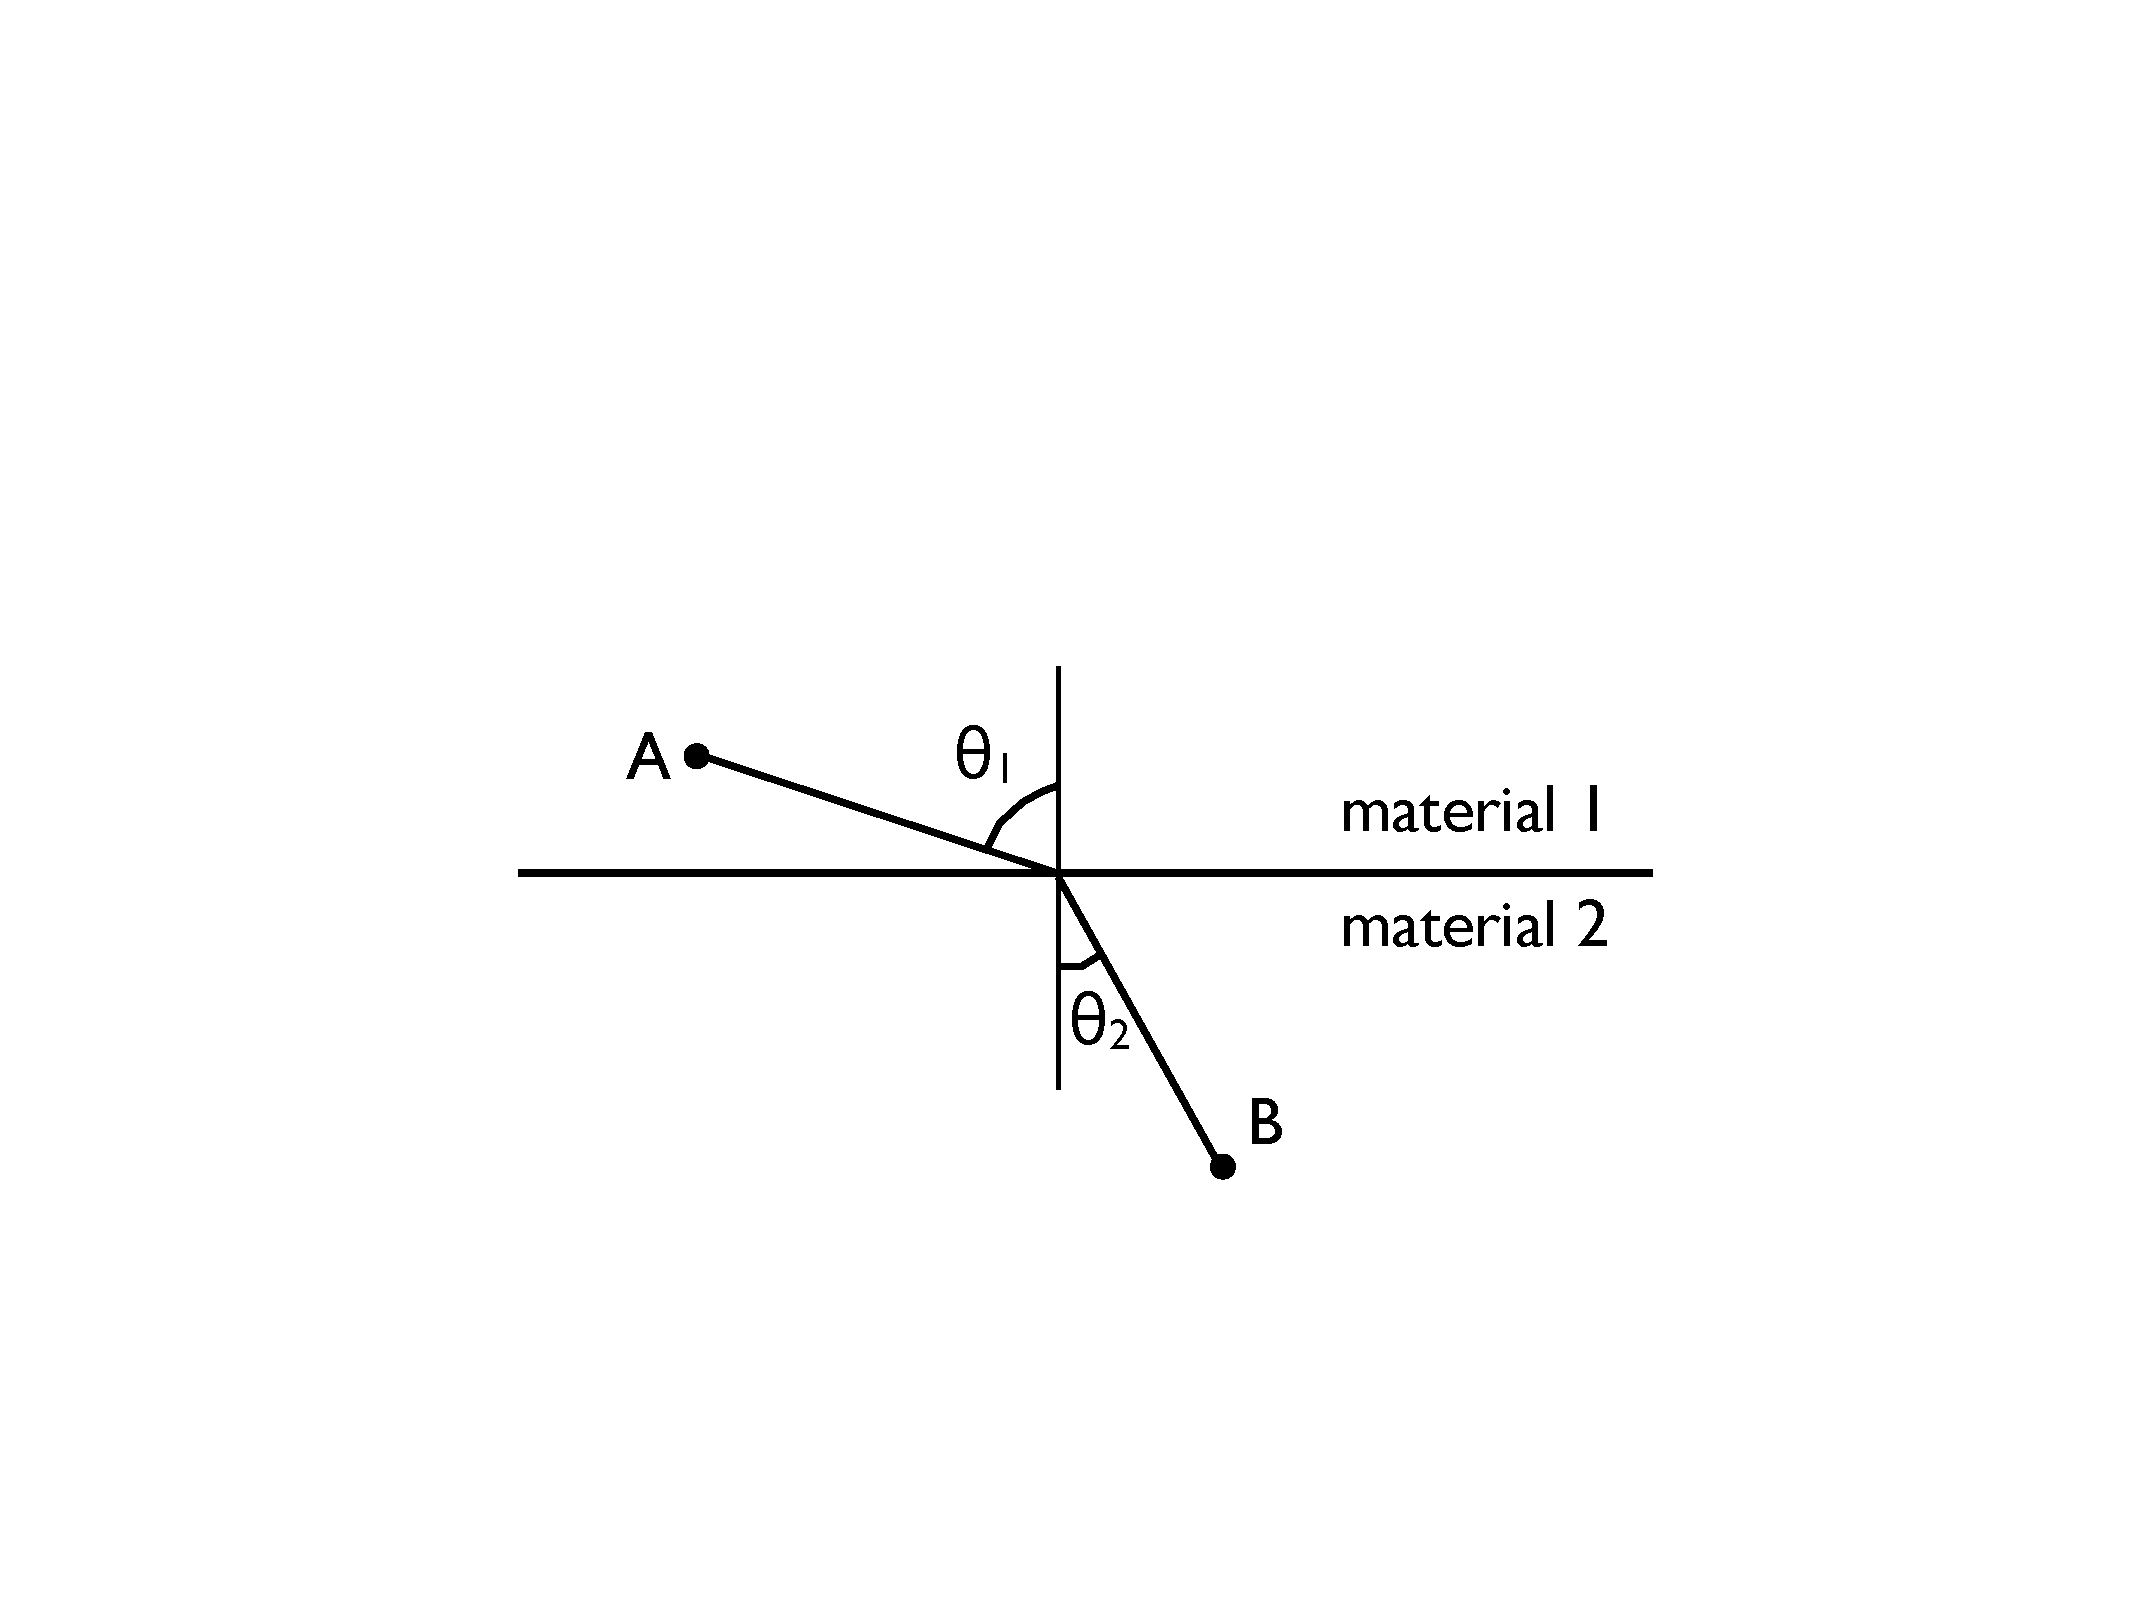
\includegraphics[width=4in]{refraction}
  \caption{Incident and refracted rays.}
  \label{f:refraction}
  \end{center}
\end{figure}

\i \ex Surface water waves tend to approach the shore 
at right angles, regardless of the initial direction
of propagation far from the shore.
This is because the velocity 
of the waves decreases as the water becomes more shallow
closer to the shore.
(Treat the water as a succession of media with 
different wave velocities, and then apply
Snell's law to each successive interface to determine
the direction of propagation.)

\i \ex A similar analysis can be applied to sound waves
in air above the surface of the Earth.
If the temperature of the air decreases with 
increasing altitude, so that the velocity of 
sound in air decreases with increasing altitude, then 
sound waves will tend to propagate upward to higher 
altitudes.
For this case, it will be difficult
to hear sounds at large distances from the source.

\i \ex
Conversely, if the temperature of the air increases
with increasing altitude (called {\em temperature 
inversion}), so that the velocity of 
sound in air increases with increasing altitude, then 
sound waves will tend to propagate back toward the
surface of the Earth.
(This condition is called {\em temperature inversion}.)
For this case, one can hear sounds at relatively large
distances from the source, since the sound tends to
stay close to the surface of the Earth.

\i Wind: 
Suppose the air temperature doesn't change with 
altitude, but there is a wind blowing (i.e., the air 
has a velocity) parallel to the surface of the Earth.
Due to frictional effects, the air velocity will 
be smallest near the surface of the Earth; 
it will increase with increasing altitude.

Since the air is moving relative to the ground,
the relevant sound speed is the {\em speed of sound 
with respect to the ground}, not with respect to 
the air.

\i \ex For sound propagating in the same direction 
as the wind, the velocity of sound with respect to the ground 
increases with altitude, similar to the temperature inversion case.
{\em Thus, it is easy to hear sound that propagates 
in the direction of the wind.}

\i \ex For sound propagating in the direction opposite 
to the wind, the velocity of sound with respect to the ground 
decreases with altitude, similar to 
the case where the air temperature decreases with altitude.
{\em Thus, it is difficult to hear sound that propagates
against the wind.}


\ei
%%%%%%%%%%%%%%%%%%%%%%%%%%%%%%%%%%%%%%%%%%%%%%%%%%%%%%%%%
\subsection{Diffraction}
\bi

\i Diffraction refers to the `spreading' of a wave as
it passes through an opening or around an obstacle 
in space.

\i For a fixed size object, diffraction is most noticeable
for waves that have wavelengths comparable to or bigger
than the size of the opening or obstacle.

\i Visible light has a wavelength ($\sim 500~{\rm nm}$)
much smaller than normal everyday objects.
Hence everday objects cast sharp shadows for visible
light, so you cannot see around a corner.

\i Sound has much larger wavelengths (a 440~Hz note
has a wavelength of about 1~m).
Hence sound waves can easily diffract through doorways
and objects less than about 100~m in size.

\i Similarly, AM radio waves (electromagnetic waves) 
have a longer 
wavelength than FM radio waves, and hence can diffract 
around large buildings better than FM waves.

\i \exer
AM radio stations broadcast with frequencies between 530~kHz and 1710~kHz;
FM radio stations broadcast with frequencies between 88~MHz to 108~MHz.
Using $v=3\times 10^8~{\rm m/s}$ for the velocity of 
electromagnetic waves in air, calculate the wavelength of a
(a) 1000~kHz AM radio wave, and 
(b) 100~MHz FM radio wave.

\ans
(a) 300~m, (b) 3~m.

\ei
%%%%%%%%%%%%%%%%%%%%%%%%%%%%%%%%%%%%%%%%%%
\subsection{Doppler effect}
\bi

\i Doppler effect:
The change in observed frequency due to the
motion of the source and/or receiver relative
to the medium through which the sound travels.

\i \ex 
The observed frequency of a siren on a police car 
that is moving toward you is larger than the 
frequency of the siren when it is at rest.
The observed frequency is smaller when the police 
car is moving away from you.

\i \demo
Use the function generator and a small speaker to
produce a pure tone, e.g., 440~Hz.
Then take the speaker, still connected to the
function generator by a long cable, and twirl it
overhead in a circle.
One can hear the frequency of the sound increase 
and decrease as the speaker approaches and recedes 
from the listener.

\ei
